\begin{refsection}
    \renewcommand{\thefigure}{\arabic{figure}}
    \renewcommand{\thetable}{\arabic{table}}
    
    \chapterOneLine
    {A importância do Espaço Escolar para o ensino-aprendizagem a luz de um estudo de caso }
    \label{chap:imprtancia-espaco-e}

    \articleAuthor
    {Ângela Maria Paulo}
    {Graduada em Gestão Pública pela Universidade Federal do Rio Grande do Norte. Especialista em Gestão e Organização Escolar pelo Instituto de Educação Superior Presidente Kennedy. ID Lattes: 6288.9301.4414.5498. ORCID: 0000-0002-3628-6501 E-mail: angella\textunderscore{}paulo@hotmail.com.}
    
    \articleAuthor
    {José Avelino da Hora Neto}
    {Licenciado em Geografia pelo Instituto Federal de Educação Tecnológica do Rio Grande do Norte e Mestre em Estudos Urbanos e Regionais pela Universidade Federal do Rio Grande do Norte. Professor Formador no Instituto de Educação Superior Presidente Kennedy. ID Lattes: 6141.3889.8327.2927. ORCID: 0000-0002-3575-3868. E-mail: avelinodahora@gmail.com.}
    
    \begin{galoResumo}
        \marginpar{
            \begin{flushleft}
            \tiny \sffamily
            Como referenciar?\\\fullcite{SelfPauloAndNeto2021importância}\mybibexclude{SelfPauloAndNeto2021importância}, p. \pageref{chap:imprtancia-espaco-e}--\pageref{chap:imprtancia-espaco-eend}, \journalPubDate{}
            \end{flushleft}
        }
        Objetiva-se com este estudo analisar a percepção da importância do espaço físico escolar como estratégia pedagógica para o ensino-aprendizagem. No decorrer da pesquisa apresenta-se noções sobre o conceito de espaço físico escolar, sua percepção pela comunidade escolar, e influência na cultura organizacional da gestão. O estudo de caso foi realizado na Escola Estadual Tiradentes, localizada na cidade de Natal/RN, numa abordagem quantitativa/qualitativa, com metodologia de natureza aplicada e caráter exploratório. Diante dos dados coletados os resultados mostram o reconhecimento da influência do espaço físico no processo de ensino-aprendizagem, as carências estruturais inerentes aos processos curriculares que nelas acontecem, assim como a percepção do espaço como uma dimensão social, cultural e simbólica.    
    \end{galoResumo}
    
    \galoPalavrasChave{Espaço físico escolar. Organização escolar. Gestão escolar.}

    \begin{otherlanguage}{spanish}

        \begin{galoResumo}[Resumén]
            El objetivo de este estudio es analizar la percepción de la importancia del espacio físico escolar como estrategia pedagógica para la enseñanza-aprendizaje. Durante la investigación se presentan nociones sobre el concepto de espacio físico escolar, su percepción por parte de la comunidad escolar y su influencia en la cultura organizacional de gestión. El estudio de caso se llevó a cabo en la Escola Estadual Tiradentes, ubicada en la ciudad de Natal / RN, en un enfoque cuantitativo / cualitativo, con metodología de carácter aplicado y carácter exploratorio. En vista de los datos recogidos, los resultados muestran el reconocimiento de la influencia del espacio físico en el proceso de enseñanza-aprendizaje, las deficiencias estructurales inherentes a los procesos curriculares que ocurren en ellos, así como la percepción del espacio como una dimensión social, cultural y simbólica.
        \end{galoResumo}
        
        \galoPalavrasChave[Palabras clave]{Espacio físico escolar. Organización escolar. Gestión escolar. }
    \end{otherlanguage}

    \section{Introdução}

    Em meio aos intensos avanços tecnológicos vivenciados pela sociedade atual, não há como não questionar as condições estruturais e materiais das escolas públicas no nosso país. Se pararmos para refletir sobre como eram as salas de aula há um século e como elas são hoje, percebemos semelhanças e ao mesmo tempo disparidades. Ao voltarmos o olhar para as salas de aula das escolas públicas, constatamos que pouco ou quase nada mudou na sua estrutura, arquitetura e organização. Além de evidenciar uma possível desconexão com a dinâmica social, esse fato nos intriga ao ponto de se fazer necessário buscar elementos que justifiquem as mesmas carteiras, as mesmas filas, os mesmos quadro e giz. 

    O espaço físico representa a materialidade, é a parte construída, elaborada, percebida. É a parte relacionada à arquitetura, a edificações, prédios, é a disposição de móveis, objetos. Quando nos referimos a esses espaços, mais especificamente ao espaço escolar, objeto do nosso estudo, imaginamos que as diversas atividades desenvolvidas exigem condições específicas para cada atividade, como exemplo as aulas de educação física ou de ciências em um laboratório. Cada aula requer espaço e movimentos específicos, principalmente se na sala existirem alunos com necessidades educacionais especiais \cite{CARPINTEROAndALMEIDA2009Teorias}. 

    O presente artigo se baseia no estudo do espaço escolar, com ênfase na relevância do espaço físico como espaço social, lugar de convivência e organização dos ambientes que se constituem em espaços de interferência direta no trabalho educativo. A pesquisa foi desenvolvida como um estudo de caso na Escola Estadual Tiradentes, localizada na Rua Régulo Tinoco, no Bairro Barro Vermelho, no município de Natal/RN. É um estudo com abordagem quantitativa/qualitativa, metodologia de natureza aplicada, de caráter exploratório; analítica e descritiva. 

    Dito isso, pretende-se contribuir com a compreensão de outros modos de percepção do espaço escolar, que para além de um espaço de transmissão do conhecimento, deve ser visto como uma organização marcada pela interação entre as pessoas, com a criação do sentimento de pertencer, pela promoção da formação humana e pela gestão democrática, tornando esses valores inerentes à prática pedagógica.  


    \section{A relevância do espaço físico escolar no processo de ensino-aprendizagem}

    A compreensão de espaço foi construída e reconstruída ao longo do tempo, evoluindo gradativamente de uma dimensão apenas geométrica para uma dimensão social, cultural e simbólica. 

    O conceito de espaço é produzido a partir das relações entre os objetos criados e as intencionalidades das ações sobre eles. Essa dinâmica é estabelecida historicamente pela sociedade, o que demonstra o surgimento de territorialidades que \textcite{SACK1986Human} define como expressões geográficas de poder, sendo um meio pelo qual o espaço e a sociedade são inter-relacionados. Verifica-se que as características do espaço são construídas socialmente por intermédio de estruturas e processos que delimitarão sua forma e função. \textcite{HORANETO2015Dinâmica} complementa essa relação observando que: 

    \begin{quotation}
        o espaço não é entendido como algo que contenha uma natureza cristalizada, impregnado de uma natureza prévia, seus significados derivam dos investimentos feitos sobre ele, por meio de técnicas onde não há espaços sem as práticas que lhe conferem sentido. \cite[p.~22]{HORANETO2015Dinâmica}. 
    \end{quotation}

    Diante disso, em seu livro \textit{A Representação do Espaço na Criança}, Piaget descreve o processo das estruturas perceptivas ou sensório-motoras, que se constituem a partir do contato direto com os objetos até a construção representativa do espaço, quando traz à lembrança a imagem do objeto em sua ausência. Na criança, as primeiras relações construídas por ela dizem respeito às características dos objetos em si mesmos, com suas relações de vizinhança, separação, envolvimento, continuidade e ordem. Este período serve de base para a construção do próximo período, quando a criança adquire os conceitos através da noção de objeto no espaço e visualiza a ideia do objeto \cite{MONTOITOAndLEIVAS2012Representação}. 

    Para Piaget \cite[apud][]{CARPINTEROAndALMEIDA2009Teorias} a relação que existe entre a noção de espaço e a de movimento, corresponde ao movimento do corpo humano, pois só percebemos o espaço para nossos movimentos quando chegamos aos limites desse espaço. Diz que “[\dots] o objeto somente se constituirá sujeitando-se ou resistindo às coordenadas dos movimentos”, pois somente aprendemos a reconhecer ou não as coisas quando conseguimos movimentá-las \cite{CARPINTEROAndALMEIDA2009Teorias}. Cabe enfatizar a relação entre a noção de espaço e a de movimento, uma vez que não existe movimento sem espaço e que o movimento está ligado ao desenvolvimento. 

    É inquestionável a importância da estrutura física da escola para o desenvolvimento das atividades inerentes ao processo de ensino-aprendizagem. É preciso uma estrutura física e pedagógica onde se possa desenvolver o currículo, uma vez que o espaço escolar exerce um carácter educacional, afetivo e cultural. 

    A escola se constitui em referência histórica ao produzir marcas boas ou más em quem por ela passa principalmente em crianças, conforme as experiências nela vividas. Nela se desenvolvem vínculos afetivos e sentimento de pertencimento, como também conhecimento e familiaridade com as questões escolares, principalmente quando há a participação da comunidade. Para \textcite[p.~81]{SANTOS2014Espaço}, “quando o homem se defronta com um espaço que não ajudou a criar, cuja história desconhece, cuja memória lhe é estranha, esse lugar é a sede de uma vigorosa alienação”. 

    Nessa condição, o edifício escolar assume um papel de destaque na memória de quem por ele passa, tendo em vista que a partir da contribuição para a transformação daquele espaço, também se torna parte dele e se reconhece como integrante ativo da cultura organizacional da escola e participante do processo de ensino-aprendizagem. É fundamental, também, discutir ações que remetam a uma reflexão do papel pedagógico do espaço escolar como suporte físico da educação, dada a importância que tem como realidade social e material, dentro da história da escola.  

    Já na década de 1930, Anísio Teixeira, então diretor da Instrução Pública do Distrito Federal, demonstrava preocupação com a qualidade e com a inexistência de prédios para as escolas públicas, já que as poucas escolas funcionavam em residências, muitas em ruínas e sem material didático e mobiliário adequado. Em debates sobre a temática, Anísio Teixeira destacava a importância e a necessidade do prédio escolar para o sistema educacional, para ele:

    \begin{quotation}
        Existe uma relação de causa e efeito, de meios e fins, entre o prédio e a instalação escolar, de um lado, e o programa e os fins da educação, de outro lado. Pelos prédios e instalações escolares e não pelas leis e regulamentos é que se pode conhecer o verdadeiro programa de ensino de uma localidade. [\dots] Prédios e instalações é que fixam os limites e marcam as diretrizes de um sistema escolar \cite[p.~5--6]{TEIXEIRA1934Problema}.
    \end{quotation}

    Com isso, percebemos que para o desenvolvimento das atividades educacionais, há a necessidade de um espaço físico que propicie uma cultura organizacional própria, proporcionando, ao educando e aos educadores, um espaço propício ao sucesso do processo de ensino aprendizagem. 


    \section{Espaço escolar e cultura organizacional}

    A escola é uma organização social, um organismo vivo, inacabado, onde cada um que por ela passa deseja dar e receber uma contribuição das experiências adquiridas no cotidiano. A escola tem propósitos definidos, embora não seja definitiva, uma vez que está em constante evolução, em busca de promover a aprendizagem da cidadania, mediante a compreensão do mundo pelo aluno, de si mesmo e de seu papel nesse mundo, além de vivências de experiências sociais significativas \cite{LÜCK2011Gestão}. Sendo assim, a cultura organizacional escolar está relacionada ao conceito de espaço, uma vez que nele são compartilhados conhecimentos e valores de um determinado tempo. 

    A cultura organizacional corresponde ao conjunto de tradições, crenças, conhecimentos, valores transmitidos de uns para os outros através de comportamentos, atitudes, discursos, relatos de histórias, comumente sem consciência por quem passa e por quem recebe. A cultura organizacional da escola se refere ao seu modo de ser e de fazer, a peculiaridade e singularidade do estabelecimento de ensino. Assim, o uso e o cuidado com os espaços, a disposição e o uso de materiais indicam por seus profissionais o que pretendem reforçar e orientar \cite{LÜCK2011Gestão}. 

    O modo como o gestor escolar conduz a organização da escola revela traços da sua cultura. Para \textcite{LÜCK2011Gestão}, é na gestão dos processos de comunicação e de relacionamento interpessoal organizados pela coletividade escolar com responsabilidade social, constituída por um ambiente voltado para a formação e aprendizagem dos alunos que se efetiva o trabalho educacional com significado social na escola.  

    Toda a ação interativa, interpessoal ou direta que ocorre na escola, envolvendo os educandos e os educadores, acontece nos ambientes construídos. A atratividade e a disponibilidade da infraestrutura física da escola colaboram para que essas ações tenham sucesso. Tais condições não somente favorecem a maior permanência das pessoas na escola, mas, sobretudo, tornam–na um ponto de atração, isto é, um lugar agradável e apropriado ao prazer dos educadores e educandos \cite{CARPINTEROAndALMEIDA2009Teorias}. 

    A cultura escolar assume as características das pessoas pelas quais é formada e ao contrário do que se possa imaginar ela não é fixa, nem permanente, ela é um processo social dinâmico, está em constante transformação, ou seja, será conservadora, inovadora ou promissora se as pessoas assim o forem, assim: 

    \begin{quotation}
        [\dots] a direção da escola pode promover a criação de uma cultura organizacional, de um clima favorável, de relações de confiança, como condições para melhor funcionamento da organização. [\dots] a cultura da escola pode ser modelada, planejada, conformada para atender aos objetivos da direção, como a coesão e o espírito grupal. [\dots] vai além de um sistema de gestão baseado apenas na autoridade do diretor e nos procedimentos burocráticos. \cite[p.~93]{LIBÂNEO2015Organização}. 
    \end{quotation}

    Portanto, a cultura organizacional escolar pode ser aprimorada por seus membros conforme a necessidade da comunidade e “a partir da interação entre diretores, coordenadores, professores, funcionários e alunos a escola vai adquirindo, na vivência do dia a dia, traços culturais próprios, vai formando crenças, valores, significados, modos de agir, práticas” \cite[p.~94]{LIBÂNEO2015Organização}. 


    \section{Espaço escolar e currículo}

    A própria palavra currículo, ato de correr, percurso, remete para o caráter espacial dessa ferramenta escolar. Considerando o aspecto espacial da escola, o termo currículo pode ser definido como “uma ambientação para vivenciar experiências culturais” \cite[p.~129]{LIBÂNEO2015Organização}, já que é no ambiente escolar onde ocorre o processo educativo. Porém, adotaremos a seguinte definição de currículo: 

    \begin{quotation}
        O conjunto dos conteúdos cognitivos e simbólicos (saberes, competências, representações, tendências, valores) transmitidos (de modo explícito ou implícito) nas práticas pedagógicas e nas situações de escolarização, isto é, tudo aquilo a que poderíamos chamar de dimensão cognitiva e cultural da educação escolar. \cite[FORQUIM, 2000, p.~48, apud][p.~129]{LIBÂNEO2015Organização}. 
    \end{quotation}

    Assim como o espaço escolar, “o currículo nunca é apenas um conjunto neutro de conhecimentos” \cite[p.~59]{APPLE1992The}, ele “comunica princípios essenciais de uma proposta educativa” \cite[PEDRA, 1997, apud][p.~129]{LIBÂNEO2015Organização}. Assim como o espaço físico, o currículo também transmite valores, princípios estéticos, éticos e políticos através da sua organização e na constituição de uma cultura escolar. 

    Constituído como lugar de aprendizagem, a arquitetura do prédio e seus elementos simbólicos, a localização das escolas nas cidades, a disposição das salas de aulas e de outras instalações, o tipo e a disposição das carteiras e dos móveis, não são elementos neutros na educação. Todos esses aspectos, desde a estrutura arquitetônica do prédio ao mínimo detalhe decorativo, devem ser considerados como também fazendo parte do currículo escolar. 

    Os espaços educativos estão repletos de significados e transmite uma importante quantidade de estímulos, conteúdos e valores que embora não estejam explícitos afetam a vida das pessoas. Libânio (2015, p. 143), afirma que o currículo oculto, está “oculto” porque não aparece no planejamento, embora se constitua como importante fator de aprendizagem,

    \begin{quotation}
        [\dots] representa tudo o que os alunos aprendem pela convivência espontânea, em meio as várias práticas, atitudes, comportamentos, gestos, percepções que vigoram no meio social e escolar. [\dots] ele segue uma sequência que começa quase sempre na esfera política e administrativa do sistema escolar, passa pelas crenças, significados, valores, comportamentos existentes na cultura, é retrabalhado pelos professores, até chegar aos alunos. \cite[p.~143]{LIBÂNEO2015Organização}. 
    \end{quotation}

    O currículo por não ser neutro, resulta de uma seleção feita por alguém com uma visão do que é o verdadeiro conhecimento, ou do que seja o conhecimento legítimo. É produto de tensões, conflitos e concessões culturais, políticas e econômicas que organizam e desorganizam um povo. O que é valido como conhecimento e considerado apropriado para aprendizagem está diretamente relacionado à maneira como domínio e subordinação são reproduzidos na sociedade, assim: 

    \begin{quotation}
        Sempre existe uma política do conhecimento oficial, uma política que exprime o conflito em torno daquilo que alguns veem simplesmente como descrições neutras do mundo e outros, como concepções de elite que privilegiam determinados grupos e marginalizam outros. \cite{APPLE1992The}. 
    \end{quotation}

    Esse aspecto é igualmente ressaltado por Paulo Freire ao criticar instituições educacionais tradicionais, quando diz que: 

    \begin{quotation}
        numa sociedade de classes, são as elites do poder, necessariamente, as que definem a educação e, consequentemente, seus objetivos. E estes objetivos não podem ser, obviamente, endereçados contra os seus interesses \cite[FREIRE, 1976, p.~116, apud][p.~101]{BEISIEGEL2010Paulo}.
    \end{quotation}

    Não é de hoje os conflitos e questionamentos sobre o que deve e o que não deve ser ensinado, pois além de ser uma questão educacional é também, ideológica e política.  


    \section{Metodologia e informações sobre a escola pesquisada}

    O presente estudo foi desenvolvido numa abordagem quantitativa/qualitativa, metodologia de natureza aplicada, de caráter exploratório; analítica e descritiva, tendo como referencial para o percurso metodológico \textcite{LavilleAndDionne1999Construcao}. O trabalho de pesquisa constituiu-se em fazer uma análise sobre a relação entre a utilização dos espaços escolares como ambientes de aprendizagem para os estudantes do ensino fundamental anos finais. Para isso, partimos da seguinte pergunta: \textit{O espaço escolar exerce influência no processo de ensino-aprendizagem?} Como instrumentos de coleta de dados, utilizamos respectivamente os seguintes:

    \begin{enumerate}
        \item Observação do ambiente escolar; 
        \item Entrevista;  
        \item O questionário com perguntas abertas e fechadas. 
    \end{enumerate}

    Os instrumentos foram aplicados em diferentes integrantes da comunidade escolar divididos em dois grupos. O primeiro engloba os profissionais da educação, entre eles professores do ensino fundamental, funcionários e equipe gestora, o segundo compreende estudantes do 6º aos 9º anos. 

    A organização dos dados permite a criação de possibilidades e diferentes caminhos para posterior análise do material coletado. \textcite{LavilleAndDionne1999Construcao} citam que esse momento de planejamento (seleção e organização dos dados) da pesquisa comporta três operações principais: codificação, transferência e verificação. Para a análise dos dados coletados na pesquisa, foram realizados procedimentos de análise qualitativa e quantitativa. \textcite{LavilleAndDionne1999Construcao} explicitam que a abordagem qualitativa na análise de dados possibilita perceber as inferências, o sentido que está entre as categorias chave e a relação entre essas categorias. 

    A Escola Estadual Tiradentes funciona desde 1976, fica na Rua Régulo Tinoco, no Bairro Barro Vermelho, localizado na zona leste do município de Natal/RN, em um amplo terreno cercado em todo o seu perímetro por um muro. É um bairro cuja paisagem é constituída por prédios e casas bem construídos que demonstram um melhor nível econômico dos moradores. Muitos dos alunos que se matriculam na escola vêm de outros bairros, e até de outros municípios.  

    A escola em questão é direcionada para o ensino fundamental e funciona nos turnos matutino e vespertino e conta com 15 salas de aula, 1 sala de professores, o setor de secretaria possui uma sala com uma divisão em mais 2 salas de arquivos, 1 diretoria, 1 sala de recursos multifuncionais para Atendimento Educacional Especializado, 1 cozinha, 1 biblioteca, sanitários, sanitário adequado a alunos com deficiência ou mobilidade reduzida, banheiro com chuveiro, 1 refeitório, 1 despensa, 2 almoxarifados, 1 auditório, 1 sala de vídeo, 1 coordenação, dependências e vias adequadas a alunos com deficiência ou mobilidade reduzida, 1 quadra de esporte descoberta, pátio descoberto, área verde, estacionamento. 

    A conservação das estruturas é razoável graças ao trabalho de manutenção do prédio e conscientização dos alunos para manter a escola sem pichação. As condições de funcionamento do prédio são consideradas boas, mas os equipamentos escolares são bastante precários: ausência de laboratórios de ciências e informática, falta de uma quadra coberta para a prática de Educação Física. A escola possui rampas para alunos que fazem uso da cadeira de rodas, que dão acesso a dependências essenciais da escola, mas não tem corrimão nem sinalizações sonora e tátil. Seu quadro funcional é composto por 52 pessoas, sendo 1 diretora, 1 vice-diretor, 6 auxiliares de secretaria, 4 coordenadoras, 2 porteiros, 2 merendeiras, 4 serventes e 32 professores. 


    \section{Resultados e discussões}

    As entrevistas foram realizadas no dia 25 de março de 2019, nos turnos matutino e vespertino com 20 profissionais, entre eles professores do ensino fundamental, funcionários e equipe gestora, e também com 30 estudantes do 6º aos 9º anos. 

    Para coleta e análise dos dados da pesquisa foi elaborado e utilizado um roteiro de entrevista com 08 questões e espaço para sugestões e opiniões, das quais 5 foram aplicadas aos professores do ensino fundamental, funcionários e equipe gestora (sendo 3 questões fechadas e 2 abertas) e 3 foram aplicadas aos estudantes do 6º aos 9º anos (sendo 2 questões fechadas e 1 aberta).  

    Conforme os dados coletados no questionário realizado com o corpo técnico-administrativo e docente da Escola Estadual Tiradentes, na pergunta inicial, como mostra a Figura \ref{fig:q1-result}, constatamos que a totalidade dos entrevistados afirma que o espaço físico exerce influência no ensino-aprendizagem.

    %% Gráfico 1

    \begin{figure}[hb]
        \caption{O espaço escolar exerce influência no ensino-aprendizagem?}
        \label{fig:q1-result}
        \centering
        
\begin{tikzpicture}[
            yes/.style={rectangle, fill=blue!50, minimum width=10cm, minimum height=1.5cm, anchor=south west}
        ]
            \node(yesnode) at (0,0) [yes] {\begin{tabular}{c} Sim \\ 100\% \end{tabular}};
            \draw[black] (0,0) rectangle (10cm,1.5cm);
        \end{tikzpicture}
        \caption*{Fonte: Elaboração da autora}
    \end{figure}


    Conforme a Figura \ref{fig:q2-result}, a maioria, totalizando 95\% consideram que o espaço físico propicia o pensamento crítico dos estudantes, enquanto 5\% acreditam que não. 

    %% Gráfico 2

    \begin{figure}[ht]
        \caption{O espaço físico da escola propicia a aprendizagem e o pensamento crítico?}
        \label{fig:q2-result}
        \centering
        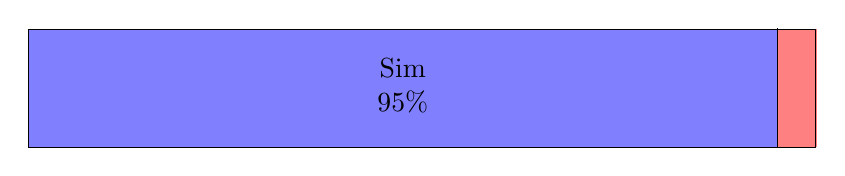
\begin{tikzpicture}[
            yes/.style={rectangle, fill=blue!50, minimum width=9.5cm, minimum height=1.5cm, anchor=south west},
            no/.style={rectangle, fill=red!50, minimum width=.5cm, minimum height=1.5cm, anchor=south west},
        ]
            \node(yesnode) at (0,0) [yes] {\begin{tabular}{c} Sim \\ 95\% \end{tabular}};
            \node[no](nonode) at (yesnode.south east) {};
            \draw[black] (0,0) rectangle (10cm,1.5cm);
            \draw[black] (yesnode.north east) -- (yesnode.south east);
        \end{tikzpicture}
        \caption*{Fonte: Elaboração da autora}
    \end{figure}

    De acordo com o Figura \ref{fig:q3-result}, quando questionados quanto à qualidade do espaço físico da escola, 60\% dos respondentes afirmam não ser o adequado e para 40\% o espaço físico é o ideal.  

    %% Gráfico 3

    \begin{figure}[ht]
        \caption{A escola, o espaço físico é adequado?}
        \label{fig:q3-result}
        \centering
        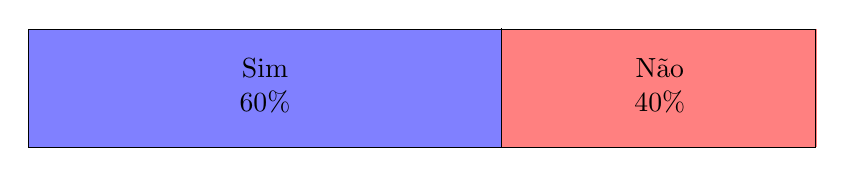
\begin{tikzpicture}[
            yes/.style={rectangle, fill=blue!50, minimum width=6cm, minimum height=1.5cm, anchor=south west},
            no/.style={rectangle, fill=red!50, minimum width=4cm, minimum height=1.5cm, anchor=south west},
        ]
            \node(yesnode) at (0,0) [yes] {\begin{tabular}{c} Sim \\ 60\% \end{tabular}};
            \node[no](nonode) at (yesnode.south east) {\begin{tabular}{c} Não \\ 40\% \end{tabular}};
            \draw[black] (0,0) rectangle (10cm,1.5cm);
            \draw[black] (yesnode.north east) -- (yesnode.south east);
        \end{tikzpicture}
        \caption*{Fonte: Elaboração da autora}
    \end{figure}

    Quando questionados se \textit{o modo como o espaço físico é organizado interfere no trabalho educativo} (pergunta 4), constatamos que a maioria concorda que haja um espaço organizado de forma acessível e atraente e que venha a atender as necessidades dos alunos e professores, pois acreditam que conforme a organização do espaço escolar o aluno pode elaborar e construir uma imagem positiva e afetiva e projetá-la para o seu futuro através do desejo de uma sociedade melhor. 

    Ainda sobre o modo como o espaço físico é organizado, para os respondentes, o ambiente escolar, para além do que se espera, ou seja, que seja limpo, amplo, arejado, bem iluminado, espera-se que seja propício e favorável ao desenvolvimento das rotinas de ensino-aprendizagem planejadas. Uma professora do ensino fundamental II considera que “todos os sentidos e percepções humanas são acionados dentro do processo de construção do conhecimento, um espaço escolar pensado e organizado para atingir tais potencialidades contribui para esse processo”. 

    Para avaliação da utilização do espaço físico pela comunidade escolar, os professores, funcionários e equipe gestora foram questionados \textit{sobre como o espaço físico poderia ser melhor utilizado pela comunidade escolar} (pergunta 5). Verificou-se que há uma certa dificuldade em compreender como se daria essa participação da comunidade no ambiente escolar, principalmente quando se referem aos pais, pois não os colocam como sujeitos ativos, capazes de também contribuir com o processo educativo.  

    A maioria das respostas colocam os pais como membros dessa comunidade, mas que a sua participação se dá apenas no sentido de receber algum serviço ou benefício da escola, como cursos, oficinas, palestras, eventos, projetos, sem uma contrapartida dos pais, como se eles fossem incapazes de oferecer alguma contribuição e colaborar de forma efetiva com a formação dos próprios filhos. 

    De acordo com os dados coletados entre os estudantes da Escola Estadual Tiradentes, como podemos observar as Figuras \ref{fig:q4-result} e \ref{fig:q5-result}, quando questionados em relação a sua satisfação com a estrutura física da escola, 80\% dos respondentes afirmam estarem satisfeitos, embora saibamos que a maioria sempre estudou nesta escola ou em escola em estado de conservação inferior e/ou com menor oferta recursos educacionais. Sendo assim, não tenha parâmetro para avaliar o que seria uma escola considerada satisfatória e que atendesse a todas as suas necessidades de estudante. Em seguida quando perguntados se acrescentariam ou mudariam alguma coisa na escola, 73\% afirmam que sim.  

    %% Gráfico 4

    \begin{figure}[ht]
        \caption{Com relação ao espaço escolar, você está satisfeito com a estrutura física desta escola?}
        \label{fig:q4-result}
        \centering
        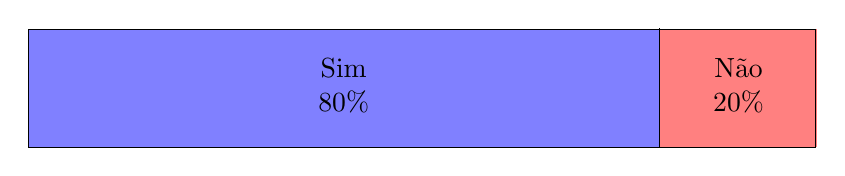
\begin{tikzpicture}[
            yes/.style={rectangle, fill=blue!50, minimum width=8cm, minimum height=1.5cm, anchor=south west},
            no/.style={rectangle, fill=red!50, minimum width=2cm, minimum height=1.5cm, anchor=south west},
        ]
            \node(yesnode) at (0,0) [yes] {\begin{tabular}{c} Sim \\ 80\% \end{tabular}};
            \node[no](nonode) at (yesnode.south east) {\begin{tabular}{c} Não \\ 20\% \end{tabular}};
            \draw[black] (0,0) rectangle (10cm,1.5cm);
            \draw[black] (yesnode.north east) -- (yesnode.south east);
        \end{tikzpicture}
        \caption*{Fonte: Elaboração da autora}
    \end{figure}

    %% Gráfico 5

    \begin{figure}[ht]
        \caption{Você acrescentaria ou mudaria alguma coisa nas instalações físicas desta escola?}
        \label{fig:q5-result}
        \centering
        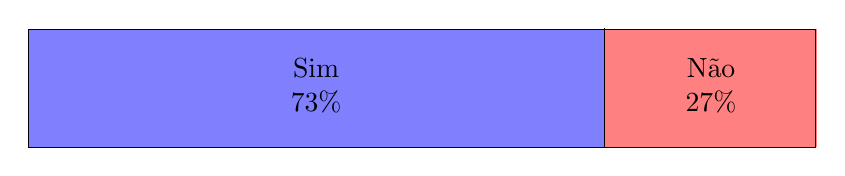
\begin{tikzpicture}[
            yes/.style={rectangle, fill=blue!50, minimum width=7.3cm, minimum height=1.5cm, anchor=south west},
            no/.style={rectangle, fill=red!50, minimum width=2.7cm, minimum height=1.5cm, anchor=south west},
        ]
            \node(yesnode) at (0,0) [yes] {\begin{tabular}{c} Sim \\ 73\% \end{tabular}};
            \node[no](nonode) at (yesnode.south east) {\begin{tabular}{c} Não \\ 27\% \end{tabular}};
            \draw[black] (0,0) rectangle (10cm,1.5cm);
            \draw[black] (yesnode.north east) -- (yesnode.south east);
        \end{tikzpicture}
        \caption*{Fonte: Elaboração da autora}
    \end{figure}

    Na Tabela \ref{tble:poll-results}, que se refere à pergunta 3, explica-se os resultados obtidos dos alunos quando questionados em relação ao modelo de escola (espaço físico) dos seus sonhos.

    %% Tabela 1
    \begin{table}
        \centering
        \caption{Qual o modelo de escola (espaço físico) dos seus sonhos?}
        \label{tble:poll-results}

        \begin{tabular}{l c}
        \toprule
        Respostas obtidas                                          & \% \\
        \midrule
        Ter quadra coberta para praticar Educação Física           & 56 \\
        Ter laboratório de informática                             & 40 \\
        Ter laboratório de ciências                                & 10 \\
        Ter salas climatizadas                                     & 10 \\
        Ter piscina                                                &  6 \\
        Está satisfeito                                            &  6 \\
        Ter uma estrutura melhor para as pessoas com deficiência   &  3 \\
        Não sabe opinar                                            &  3 \\
        \bottomrule
        \end{tabular}

        \caption*{Fonte: Elaboração da autora}
    \end{table}

    Os resultados obtidos dos alunos expressam que, o que para eles se constitui como sonhos, são na realidade o mínimo que eles têm direito como estudantes. As respostas não são algo que se possam se classificar como “sonho”, algo fora do real, uma utopia. Se o básico fosse atendido, o que eles classificaram como sonhos seriam simplesmente o que eles teriam no dia a dia de estudantes.  

    Essa análise nos remete a Teoria da Hierarquia das Necessidades de Abraham Maslow que diz que existe uma hierarquia de necessidades, das mais básicas até as de alto nível.  À medida que cada necessidade básica é atendida, surge a próxima mais elaborada. Se a necessidade básica não é atendida ocorre uma estagnação na evolução do indivíduo \cite{CAMARGO2012Psicologia}. Então se os estudantes não têm uma quadra coberta para a prática da Educação Física e laboratórios, que são necessidades básicas e deveriam ser uma realidade nas escolas públicas, não há como sonhar em ter uma piscina. 


    \section{Considerações finais}

    Este trabalho buscou chamar a atenção para a importância do espaço físico escolar em sua visão mais crítica e subjetiva. Observa-se que o ambiente escolar faz parte do contexto educacional e interfere no sucesso escolar dos alunos e na qualidade do ensino da instituição, como também para o espaço escolar que existe além do portão da escola com a participação da sociedade, da família e do Estado na construção de espaços escolares educativos.  

    Os dados coletados mostram que na escola pesquisada, embora todos estejam conscientes da importância do espaço físico escolar na qualidade do ensino-aprendizagem, esse espaço ainda não é o ideal e apresenta deficiências em relação a sua infraestrutura. Acreditam que o espaço conforme seja organizado pode melhorar a aprendizagem e pode estimular o aluno a construir uma imagem positiva e afetiva da escola, embora não apontem de forma clara como se daria essa organização.  

    Pelo constatado, a escola é ampla e as condições de funcionamento do prédio, é percebida como boa, mas existem carências de materiais e equipamentos cuja falta pode comprometer a formação dos alunos. Destaca-se que a participação dos pais como membros da comunidade escolar se dá de forma muito tímida, uma vez que falam maiores ferramentas para sua participação no processo educativo. 

    Ressaltamos que a organização e gestão escolar, recursos físicos e materiais fazem a diferença no processo de ensino-aprendizagem. Para \textcite{LIBÂNEO2015Organização}, o ambiente escolar é considerado em sua dimensão educativa, ou seja, as formas de organização e gestão, a organização do espaço físico, são também práticas educativas. 

    Portanto, compreendemos que a escola se constitui em referência histórica ao produzir marcas boas ou más em quem por ela passa, conforme as experiências nela vividas sejam positivas ou negativas e que a construção de uma escola de boa qualidade é sem dúvida um desafio. 

    \nocite{PPPEscEstTiradentes}
    \nocite{DÓREA2013Arquitetura}
    \nocite{PARO2016Gestão}

    \printbibliography[heading=subbibliography,notcategory=fullcited]

    \label{chap:imprtancia-espaco-eend}

\end{refsection}
